\styledchapter[Hoe werkt Machine Learning?]{hoe-werkt-machine-learning}

\Gls{machine-learning} (ML) is onderdeel van het domein \gls{computer-science}. Binnen \gls{machine-learning} worden algoritmische modellen gebouwd om statistische problemen op te lossen. Dit wordt gedaan met behulp van een dataset dat verzameld is uit de echt wereld of gefabriceerd door mensen. Het model kan met behulp van de dataset een redelijk nauwkeurige voorspelling maken \cite[p.~7]{the-hundred-page-machine-learning-book}.

De termen deep learning (DL) en artificial intelligence (AI) komt vaak voor als het over ML gaat. DL is een uitbreiding van neural networks, wat weer bestaat uit een set algoritmes en is grotendeels gemodelleerd naar de hersenen \cite{ml-neural-network-nicholson}. Niet alle termen en concepten van ML zijn relevant binnen DL maar valt wel onder dezelfde paraplu.

ML is onderdeel van het AI domein. Bij AI wordt niet alleen ML toegepast, maar ook concepten zoals beredeneren, plannen en vooruitdenken en het onthouden en terug refereren. Een voorbeeld hiervan is dat een ML model kan voorspellen wat het volgende woord in een zin kan zijn, maar een AI kan beredeneren waarom de zin gebouwd is zoals het is en hoe het past binnen de context van de alinea past \cite{ml-think-about-ml-brownlee}.

\section{Hoe leert een machine learning model?}\label{sec:hoe-leert-een-machine-learning-model}
Een \gls{machine-learning} model leert met behulp van een dataset om een voorspelling te maken. Een dataset kan duizenden \glspl{machine-learning-feature-vector} (voorbeelden) bevatten, waarbij elke vector een of meerdere \gls{machine-learning-feature} (attribuut) heeft. In een voorbeeld waarbij een model moet kunnen voorspellen of een persoon kanker heeft kan een \gls{machine-learning-feature-vector} één persoon zijn en de \glspl{machine-learning-feature} het gewicht, leeftijd, lengte en of de persoon kanker heeft \cite{google-ml-terminology}.

Het model gaat langs alle \glspl{machine-learning-feature-vector} en probeert correlaties te vinden tussen de features. Op basis hiervan kan het model vervolgens een voorspelling doet met een \gls{machine-learning-feature-vector} dat het model nooit heeft gezien.

Er zijn een aantal manieren om een algoritme te laten trainen, gegroepeerd in vier vormen.

\subsection{Supervised learning}\label{subsec:supervised-learning}
Met \gls{supervised-learning} wordt een model getraind door middel van een \textbf{gelabeld} dataset. Dit betekent dat een \gls{machine-learning-feature-vector} gepaard gaat met de gewenste label.

\begin{table}[hbt!]
  \centering
  \begin{tabular}{|l|l|}
  \hline
  \textbf{Feature} & \textbf{Label} \\ \hline
  woorden, afzender, tijd van versturen&spam/geen spam\\ \hline
  \end{tabular}
  \caption{Voorbeeld gelabeld dataset}
  \label{table:voorbeeld-gelabeld-dataset}
\end{table}

Het model kan leren dat woorden zoals 'gratis' in e-mails die tussen 01:00 en 03:00 worden verstuurd vaak als spam gelabeld zijn. Er kan dan geconcludeerd worden dat als een e-mail met soortgelijke features als input word gegeven, dat het een spam e-mail is \cite{google-ml-terminology}.

\subsection{Unsupervised learning}\label{subsec:unsupervised-learning}
\Gls{unsupervised-learning} lijkt grotendeels op \gls{supervised-learning}. Het verschil is dat de \glspl{machine-learning-feature-vector} in de dataset niet gepaard zijn met een label. 

\begin{table}[hbt!]
  \centering
  \begin{tabular}{|l|l|}
  \hline
  \textbf{Feature} & \textbf{Label} \\ \hline
  woorden, afzender, tijd van versturen&?\\ \hline
  \end{tabular}
  \caption{Voorbeeld niet gelabeld dataset}
  \label{table:voorbeeld-niet-gelabeld-dataset}
\end{table}

Het doel bij \gls{unsupervised-learning} is om de data op een bepaalde manier te transformeren om er iets waardevols uit te halen. Een voorbeeld hiervan is het \textit{clusteren} van data. Hierbij wordt soortgelijke data gegroepeerd (\autoref{fig:clustering-example}). Een andere voorbeeld is \textit{dimensionality reduction} (\autoref{fig:dimensionality-reduction-example}). \Gls{machine-learning-feature} worden weggelaten om twee \glspl{machine-learning-feature} tegen over elkaar te zetten om bijvoorbeeld uitschieters te vinden \cite{the-hundred-page-machine-learning-book}.

\begin{figure}[hbt!]
    \centering
    \begin{minipage}{0.3\textwidth}
        \centering
        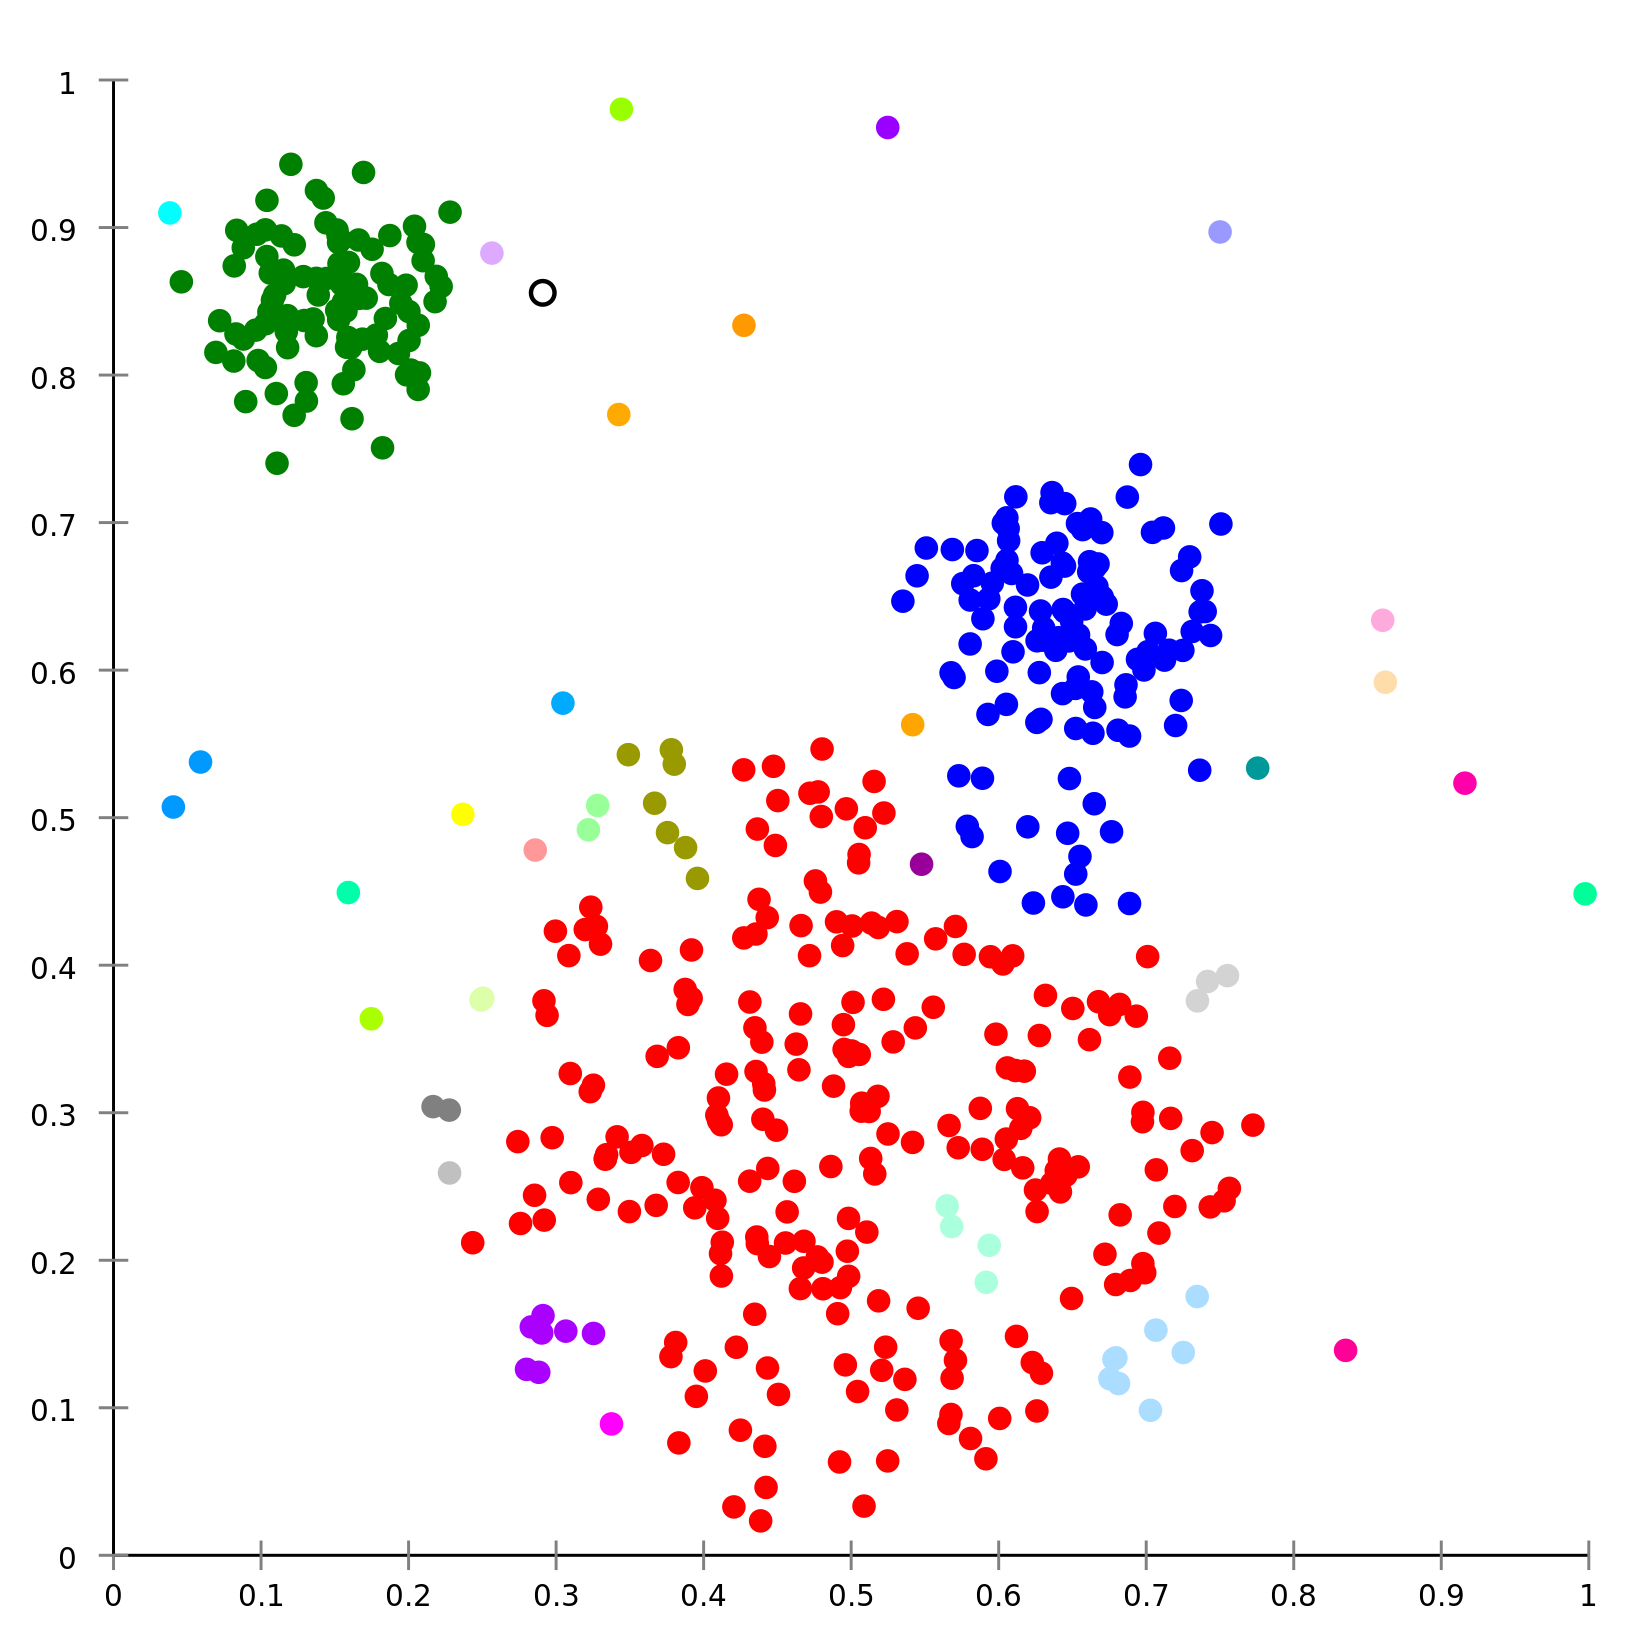
\includegraphics[width=0.9\textwidth]{./chapter-5/clustering-example.png}
        \caption{Voorbeeld van \textit{clustering}}
        \label{fig:clustering-example}
    \end{minipage}\hfill
    \begin{minipage}{0.6\textwidth}
        \centering
        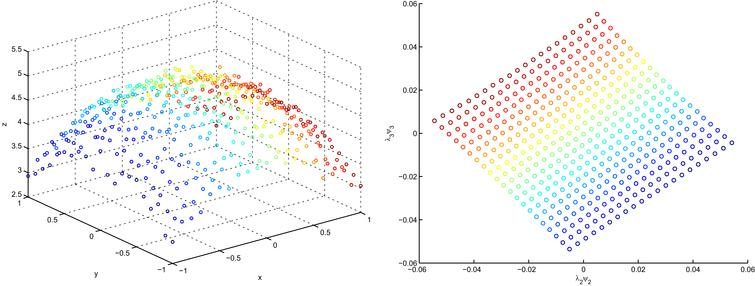
\includegraphics[width=0.9\textwidth]{./chapter-5/dimensionality-reduction-example.jpg}
        \caption{Voorbeeld van \textit{dimensionality reduction}}
        \label{fig:dimensionality-reduction-example}
    \end{minipage}
\end{figure}

\subsection{Semi-supervised learning}\label{subsec:semi-supervised-learning}
\Gls{semi-supervised-learning} is een combinatie van \gls{supervised-learning} en \gls{unsupervised-learning} waarbij het doel dezelfde is als \gls{supervised-learning}. Het is gebruikelijk dat het merendeel van de dataset niet gelabelde data is \cite{the-hundred-page-machine-learning-book}.

\subsection{Reinforcement learning}\label{subsec:reinforcement-learning}
\Gls{reinforcement-learning} wordt ook wel 'survival learning' genoemd. Een analogie hiervoor is een organisme dat moet overleven in verschillende situaties door de juiste actie te verrichten. Acties kunnen een positief of een negatief effect hebben. Acties dat langdurig een positieve effect hebben moeten versterkt worden zodat het model zo veel mogelijk positieve acties verricht \cite{bayesian-reasoning-and-machine-learning-book}.

\section{Stappenplan voor het trainen van een model}\label{sec:stappenplan-voor-het-trainen-van-een-model}
Er zijn een aantal stappen die altijd uitgevoerd moeten worden om een model te trainen, zoals: data opschonen, model trainen en een voorspelling maken met het model. Om deze stappen kunnen extra stappen geplaatst worden om de accuraatheid van de voorspelling te maximaliseren. Brownlee \cite{ml-applied-ml-process-brownlee} beschrijft een proces dat hij "Applied Machine Learning Process"\space noemt. Hierbij wordt vooraf het probleem in kaart gebracht, tussentijds gekeken welk algoritme de beste kans heeft op een hoge accuraatheid en na de selectie van het beste algoritme wordt het resultaat verbeterd als dit mogelijk is.

Het proces van Brownlee is misschien niet de beste en zeker niet de enige stappenplan. Zijn kwalificaties en toegankelijkheid van de bronnen heeft echter wel een rol gespeeld in de keuze van het leidende stappenplan en mijn eigen ervaring ondersteund de keuze.

\begin{figure}[hbt!]
  \centering
  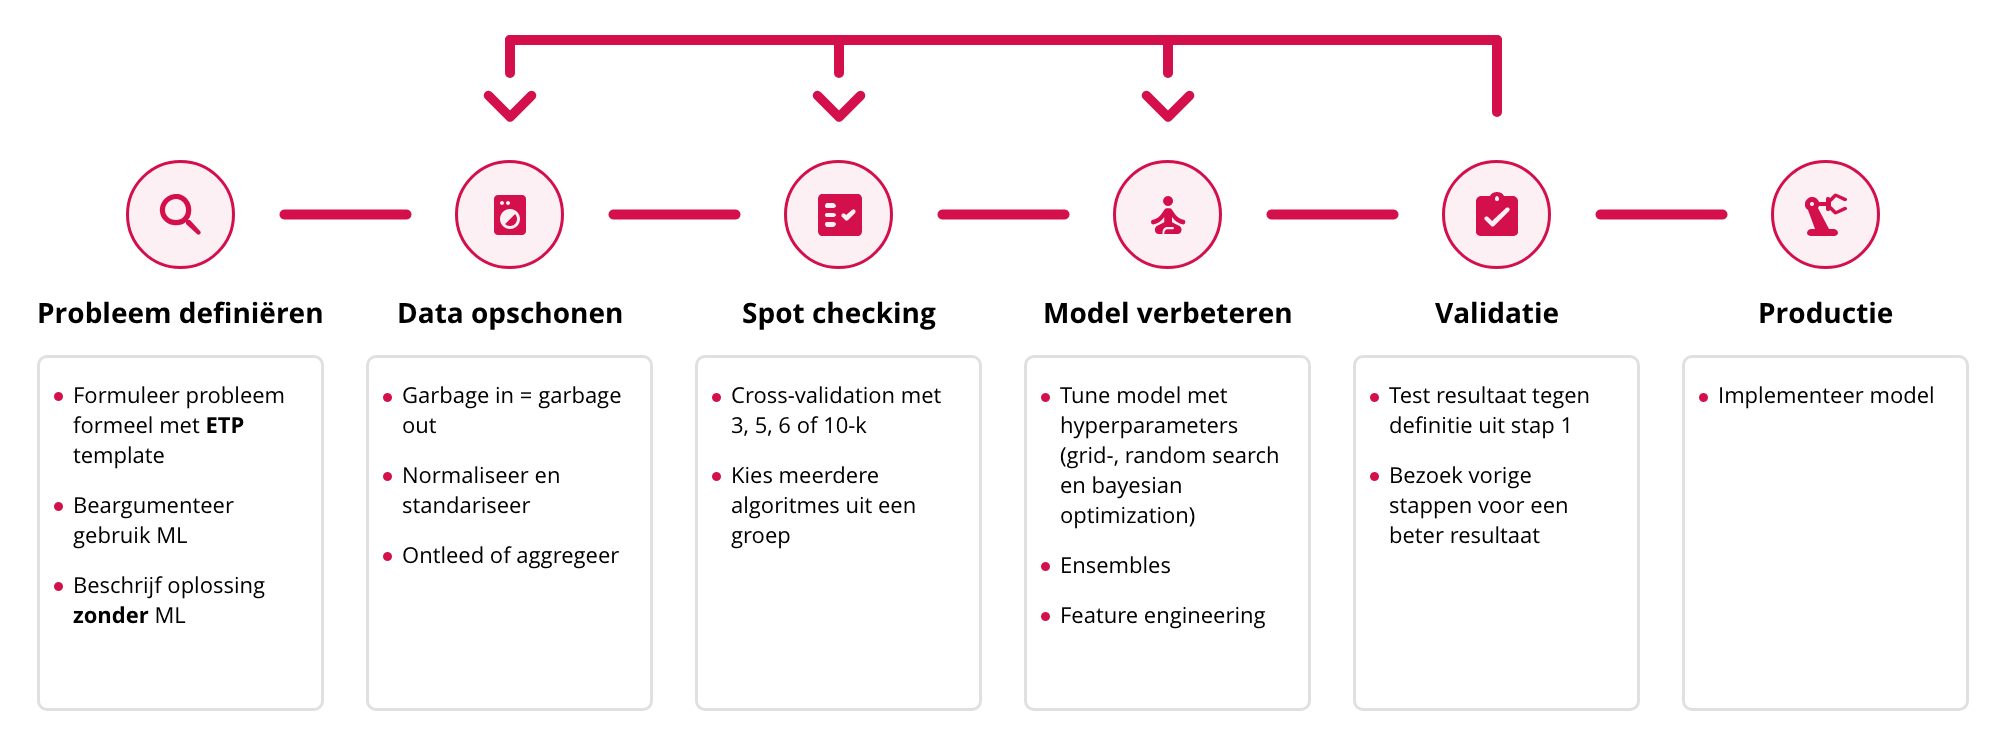
\includegraphics[width=16cm]{./chapter-5/ml-guide.png}
  \caption{Stappenplan om een model te trainen}
  \label{fig:ml-guide}
\end{figure}

\subsection{Het probleem definiëren}\label{subsec:het-probleem-definieren}
Om een ML model te trainen en het gebruik te verantwoorden, moet er gekeken worden naar \textbf{wat} het probleem is, \textbf{waarom} het een probleem is en de \textbf{hoe} het opgelost kan worden \textit{zonder} het gebruik van ML. Als eerst kan het probleem informeel geformuleerd worden, bijvoorbeeld:

\begin{quoting}
  \centering
  Ik wil het temperatuur voor de komende week voorspellen.
\end{quoting}

Informeel formuleren is wat makkelijker om mee te beginnen maar is optioneel. Nu kan het probleem formeel geformuleerd worden met behulp van Mitchells sjabloon \cite{machine-learning-mitchell}:

\begin{quoting}
  A computer program is said to learn from experience \textbf{E} with respect to some class of tasks \textbf{T} and performance measure \textbf{P}, if its performance at tasks in \textbf{T}, as measured by \textbf{P}, improves with experience \textbf{E}. 
\end{quoting}

Door de letters \textbf{E}, \textbf{T} en \textbf{P} in de zin in te vullen, kunnen we identificeren welke data er verzameld moet worden (\textbf{E}), wat het model moet kunnen doen/voorspellen (\textbf{T}) en hoe de accuraatheid gemeten kan worden (\textbf{P}).

Het informele probleem hierboven kan met behulp van Mitchells sjabloon formeel geformuleerd worden op de volgende manier:

\begin{itemize}
  \item \textbf{T}: De temperatuur voor de komende 7 dagen voorspellen
  \item \textbf{E}: De gemeten temperatuur op dagen van voorgaande jaren
  \item \textbf{P}: Hoe dicht het voorspelde temperatuur bij de gemeten temperatuur lag
\end{itemize}

Vervolgens moet er gekeken worden waarom het probleem opgelost moet worden. De motivatie achter het gebruiken van ML kan het experimenteren zijn of omdat het van je werkgever moet. De voordelen van het gebruik van ML kan ook een reden zijn. ML toepassen kan bijvoorbeeld meer tijd vrijmaken voor andere taken.

Als laatste moet een plan geformuleerd worden waarin staat hoe het probleem opgelost kan worden. In het plan kan staan wat voor data er wordt verzameld en hoe technische tekeningen er uit zien. Hierbij kunnen prototypes en experimenten bij zitten. Het is belangrijk om dit \textit{zonder} ML te doen om 'domain knowledge'\space, zoals Brownlee het noemt \cite{ml-define-ml-problem-brownlee}, naar boven te halen. Dit zijn praktische feiten zoals waar data is opgeslagen en wat voor kenmerken waardevol kunnen zijn.

\subsection{Data prepareren}\label{subsec:data-prepareren}
Bij het selecteren van de dataset is het niet verstandig alle beschikbare data te gebruiken. Meer is \textbf{niet} beter bij het trainen van een ML model. Een bekende gezegde binnen ML luid 'garbage in = garbage out'\space wat betekent dat de prestatie van het model afhangt van de kwaliteit van de dataset. Het is daarom goed om op papier te zetten wat voor data er beschikbaar is, wat er potentieel mist (en eventueel wat wel in de toekomst kan worden verzameld) en wat er niet gebruikt gaat worden.

Na de selectie moet er gekeken worden naar hoe de data gebruikt gaat worden. In deze stap wordt de data voorbewerkt. Hierbij wordt onder andere gekeken naar de formattering zoals typefouten of bestandstypes, het weghalen of repareren van missende data en het sampelen om te experimenten met een kleinere dataset zodat het snel gaat. 

Als laatste stap kan de data getransformeerd worden. Het kan zijn dat deze stap weer bezocht wordt in een later stadium om de resultaten te verbeteren. Voor veel algoritmes is het handiger om met kleine waardes te werken, zoals tussen \(0\) en \(1\). Dit heet \textit{data scaling}, of het schalen van data. Het normaliseren van data transformeert de waarde tussen \(0\) en \(1\). De formule hiervoor is:

\[y = \frac{(x - min)}{(max - min)}\]

De \(min\) is het kleinste getal in de dataset en \(max\) het grootste getal. De \(x\) is het getal wat genormaliseerd moet worden en \(y\) is het resultaat.

Een andere methode om te schalen is het standaardiseren. Hierbij wordt de verdeling van waardes herschaald zodat het gemiddelde \(0\) is en de standaardafwijking \(1\). De formule hiervoor is:

\[y = \frac{x - mean}{standard\_deviation}\]

Waarbij \(mean\) en \(standard\_deviation\) zijn:

\noindent\begin{minipage}{.4\linewidth}
    \[mean = \frac{sum(x)}{count(x)}\]
  \end{minipage}%
  \begin{minipage}{.6\linewidth}
    \[standard\_deviation = sqrt\left(\frac{sum((x - mean)^2)}{count(x)}\right)\]
\end{minipage}

Het kan voorkomen dat features te complex zijn of los niet veel betekenen, maar samen meer betekenen. Deze features kunnen \textbf{ontleed} of \textbf{geaggregeerd} worden. Een voorbeeld van ontleden is dat de datum en tijd beschikbaar zijn, maar alleen de tijd relevant is. Een voorbeeld van aggregatie is vaak voorkomend data dat in één getal dezelfde waarde heeft, zoals de aantal logins van een gebruiker \cite{ml-prepare-data-brownlee}.

\subsection{Spot check algoritmes}\label{subsec:spot-check-algoritmes}
Er zijn ontzettend veel soorten algoritmes die elke effectief kunnen zijn voor een specifiek probleem. Een algoritme heeft daar bovenop nog een aantal parameters die aangepast kunnen worden. Het is daarom niet verstandig om één algoritme te kiezen en de prestatie daarvan te verbeteren. Een effectievere manier is om een 'test harness'\space op te zetten \cite{ml-evaluate-ml-algorithm-brownlee}.

Het doel van de test harness is om snel en consistent algoritmes te testen tegen een representatie van het probleem. Met het resultaat uit de tests is het duidelijk met welke algoritme(s) het waard is om verder te gaan. Ook geeft het een idee hoe goed de dataset is en kan een algoritme accurater zijn dan eerst gedacht.

In de test harness wordt gebruik gemaakt van \gls{cross-validation}. Bij cross-validation wordt de dataset verdeeld in delen, ook wel \glspl{fold} genoemd, waarvan 1 fold een \textit{holdout} fold is. Het model wordt getraind met de folds en getest tegen de holdout fold. Dit proces wordt herhaald totdat elke fold een holdout fold is geweest. Aan het einde wordt de gemiddelde genomen van de prestatiewaarde van elke test. Het is gebruikelijk om een fold te nemen van 3, 5, 6 of 10. Een 10-k cross-validation methode is in \autoref{fig:10-k-cross-validation} gevisualiseerd \cite{ml-evaluate-ml-algorithm-brownlee}.

\begin{figure}[hbt!]
  \centering
  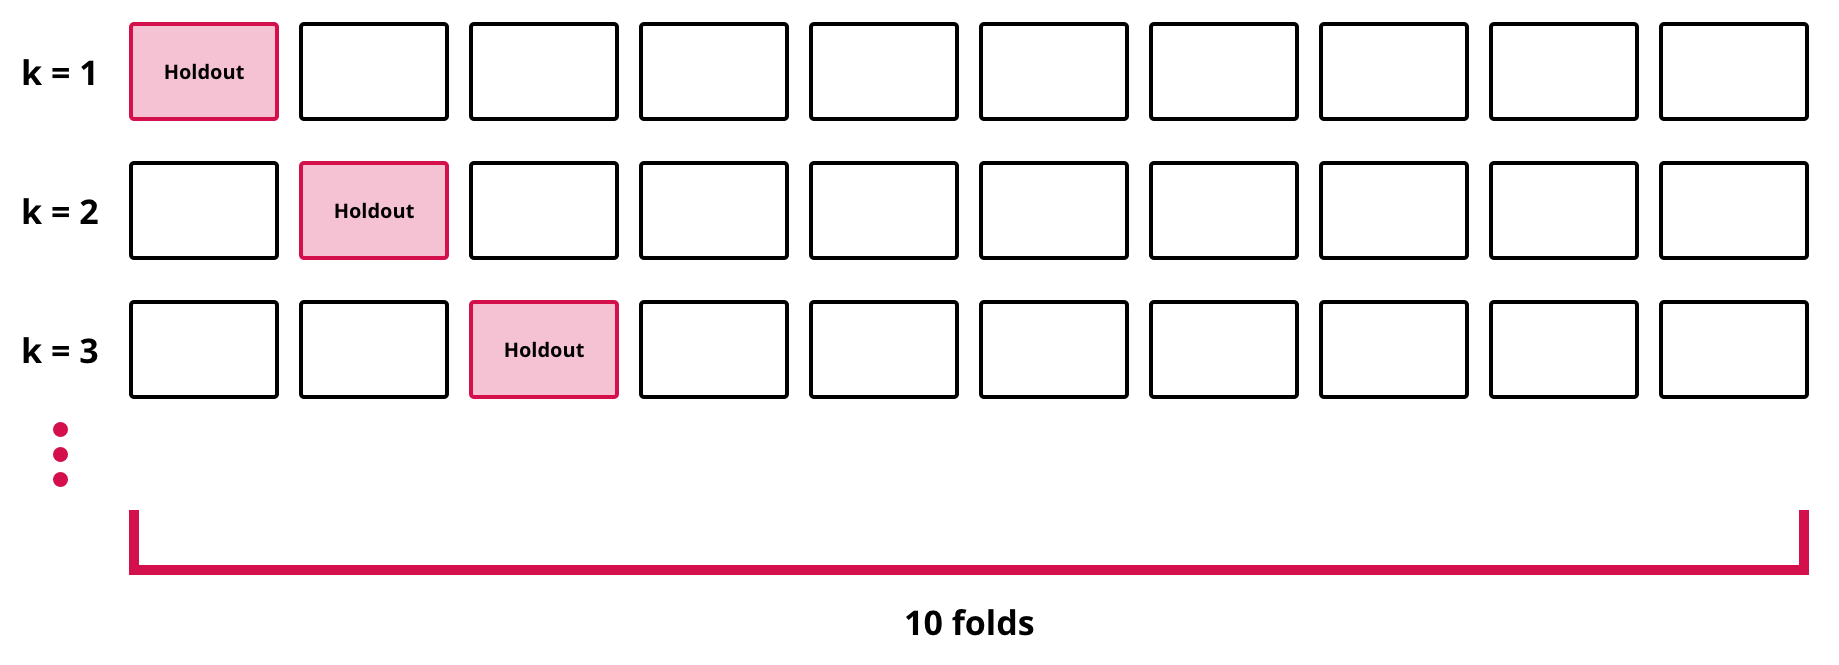
\includegraphics[width=15cm]{./chapter-5/10-k-cross-validation.png}
  \caption{Visualisatie van de 10-k cross-validation methode}
  \label{fig:10-k-cross-validation}
\end{figure}

Nu het duidelijk is wat de test harness gaat doen, kan de focus gelegd worden op welke algoritmes er wordt getest. Het is valide om één algoritme te testen, maar het is conventioneel om meerdere te testen. Algoritmes dat op dezelfde manier werken kunnen gegroepeerd worden, zoals regressie, classificatie bayesian, clustering, enz. Om te weten welke groep(en) relevant is, kan terug gerefereerd worden naar het probleem de eerste stap 1 (\autoref{subsec:het-probleem-definieren}).

\subsection{Resultaten verbeteren}\label{subsec:resultaten verbeteren}
Als laatste stap moet het model geoptimaliseerd worden. Dit kan op drie manieren. Als eerste kan het model 'getuned'\space worden wat ook wel \gls{hyperparameter-optimization} genoemd wordt. Een hyperparameter is een parameter dat wordt gebruikt om het leerproces van een model een bepaalde richting op te sturen. Er zijn een aantal manieren om de optimale waarde van een hyperparameter te achterhalen. Een aantal simpele methodes zijn grid search, random search en bayesian optimization. Met bijvoorbeeld de grid search methode wordt de minimale en maximale waarde van de parameter op een x- en y-as geplot. Deze grenzen moeten vaak zelf worden gespecificeerd. Vervolgens wordt er langs elke set gegaan en wordt doorgaans met \gls{cross-validation} de prestatie berekend. In \autoref{fig:hyperparameter-optimization-grid-search} is te zien dat de hyperparameters binnen de donkerblauwe lijnen het beste presteren. Het model presteert minder goed naarmate de lijnen rood worden.

\begin{figure}[hbt!]
  \centering
  \begin{minipage}{0.47\textwidth}
      \centering
      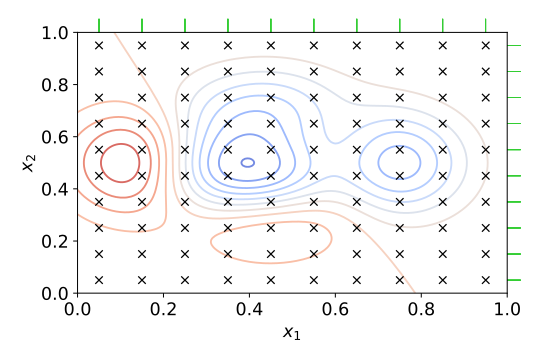
\includegraphics[width=8cm]{./chapter-5/hyperparameter-optimization-grid-search.png}
      \caption{Hyperparameter optimalisatie met de grid search methode}
      \label{fig:hyperparameter-optimization-grid-search}
  \end{minipage}\hfill
  \begin{minipage}{0.47\textwidth}
      \centering
      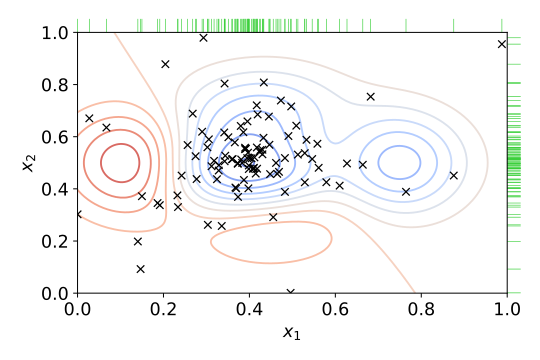
\includegraphics[width=8cm]{./chapter-5/hyperparameter-optimization-bayesian-optimization.png}
      \caption{Hyperparameter optimalisatie met de bayesian optimization methode}
      \label{fig:hyperparameter-optimization-bayesian-optimization}
  \end{minipage}
\end{figure}

Bij random search wordt hetzelfde proces doorlopen waarbij het enige verschil is dat de waardes willekeurig zijn gekozen. De bayesian optimization methode begint willekeurig, maar houd rekening met de vorige steekproeven om een keuze te maken om dichterbij of verder weg van de vorige waarde(s) te experimenteren (\autoref{fig:hyperparameter-optimization-bayesian-optimization}).

De tweede manier is met \textit{ensembles}. Bij het gebruik van ensembles wordt het resultaat van verschillende methodes bijeengevoegd om tot een beter resultaat te komen. Er zijn een aantal strategieën om dit te doen. Een daarvan is \textbf{boosting}. Hierbij worden meerdere algoritmes van dezelfde groep getraind.

Als laatste manier kan \gls{feature-engineering} gebruikt worden op de prestatie te verbeteren. De data heeft een bepaalde structuur dat het model exploiteert om een besluit of voorspelling te maken. Met \gls{feature-engineering} worden bepaalde delen van de structuur 'benadrukt'\space zodat het model de focus hierop zal leggen. Er wordt als het ware tegen het model gezegd: \say{Deze features zijn belangrijk in de keuze/voorspelling dat wordt gedaan}. Dit kan vervolgens resulteren in een accurater model.

\subsection{Validatie en productie}\label{subsec:validatie-en-productie}
Na het trainen en verbeteren van het model kan er validatie plaatst vinden. Gebruik hierbij de formulering uit stap 1 (\autoref{subsec:het-probleem-definieren}). Als het model niet of niet goed genoeg voldoet, kunnen de voorgaande stappen opnieuw bezocht worden. Als het model wel voldoet, kan het door naar productie.

\section{Kennis vereist om een model te trainen}\label{sec:kennis-vereist-om-een-model-te-trainen}
Waarom je niet alles kan voorkauwen.
Wat is de middle ground?

\section{Wachttijden voorspellen}\label{sec:wachttijden-voorspellen}


\section{Conclusie}\label{sec:conclusie}


\section{Advies}\label{sec:advies}
